\chapter{Baseline Compensation System}


\section{Basics in Seismic Isolation}\label{sec:51}
重力波望遠鏡における地面振動防振の基本は振り子である。より防振比を高めるために、低共振周波数かつ多段振り子をもちいている。


\subsection{Single Pendulum}
For simple example, as shown in left figure in Fig.(\ref{img:img501}), consider a one-dimentional harmonic oscillator consisting of a spring with a spring constant $k$ and mass $M$. The displacement of the suspension point and the mass are $x_0$ and $x$, respectively. Because the equation of the motion is written as
\begin{eqnarray} \label{eq:eq501}
  M\ddot{x} = -k(x-x_0),
\end{eqnarray}
the frequency transfer function from the displacement of the suspension point to the mass displacement $H(f)$ is given by the Fourier transform from the equation and represented as
\begin{eqnarray} \label{eq:eq502}
  H(f) \equiv \frac{1}{1-(f/f_0)^2},
\end{eqnarray}
where $f_0 = (k/M)^{1/2}$ is the resonant angular frequency of the oscillator.

According to Eq.(\ref{eq:eq502}), the amplitude of $H(f)$ is unity below the resonant frequency, the amplitude is approximately propotional to $(f/f_0)^{-2}$ above resonance frequency. The bode plot of $H(f)$ with various resonance frequencies are plotted in right figure in Fig. \ref{img:img501} . One finds that it is better to make a low-resonance frequency oscillator in order to attenuate the seismic noise broadly. 

\begin{figure}[h]
  \begin{center}   
    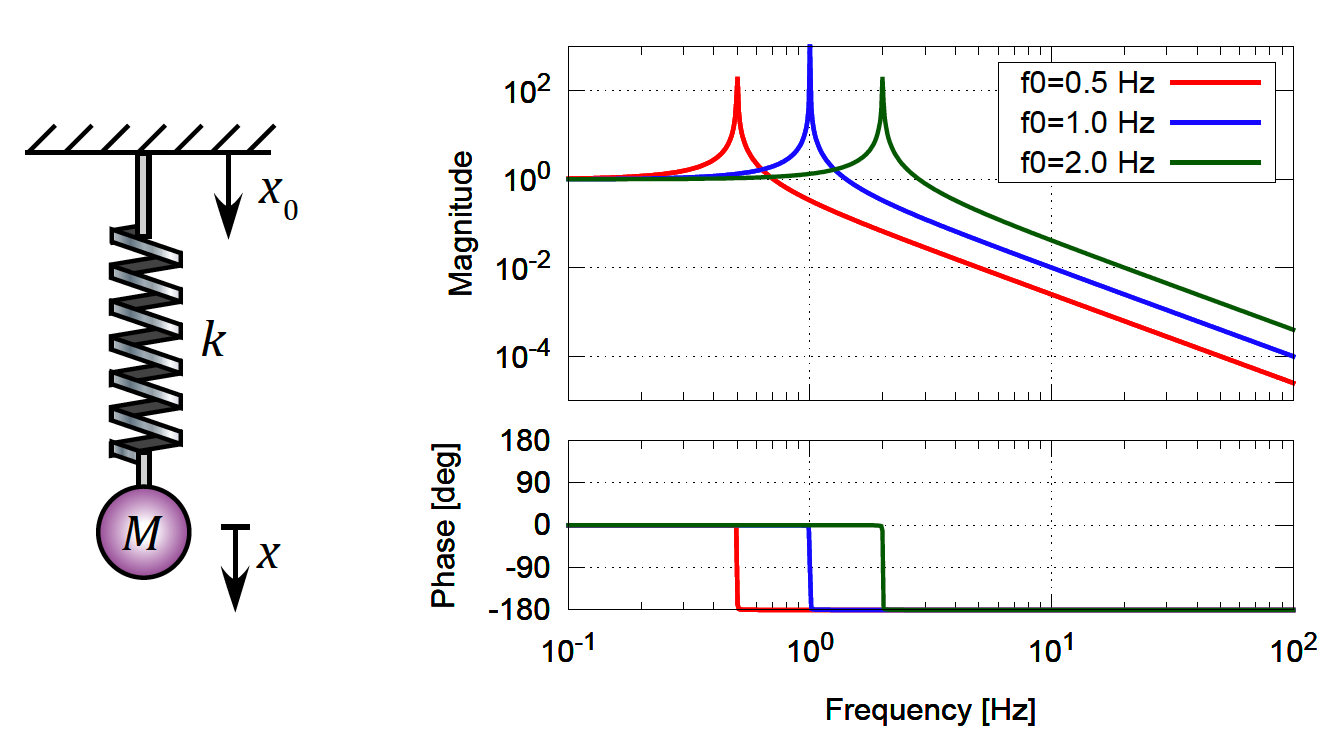
\includegraphics[width=11cm,height=6cm]{./img_chap5/img501.png}
    \caption{Single pendulum as a mechanical filter and its transfer function with various resonant frequencies. This figure is cited from Fig.(2.3) in \cite{sekiguchi2016astudy}.} \label{img:img501}
  \end{center}
\end{figure}

\subsection{Multi-stage Pendulum}
In order to increase the order of the seismic isolation, multi-stage pendulum is effective. In case of an N-stage pendulum, the transfer function from the ground to the suspended mass is propotional to $f^{-2N}$ above the resonance frequrncy of the pendulum as shown in Fig. \ref{img:img502}. 
\begin{figure}[h]
  \begin{center}   
    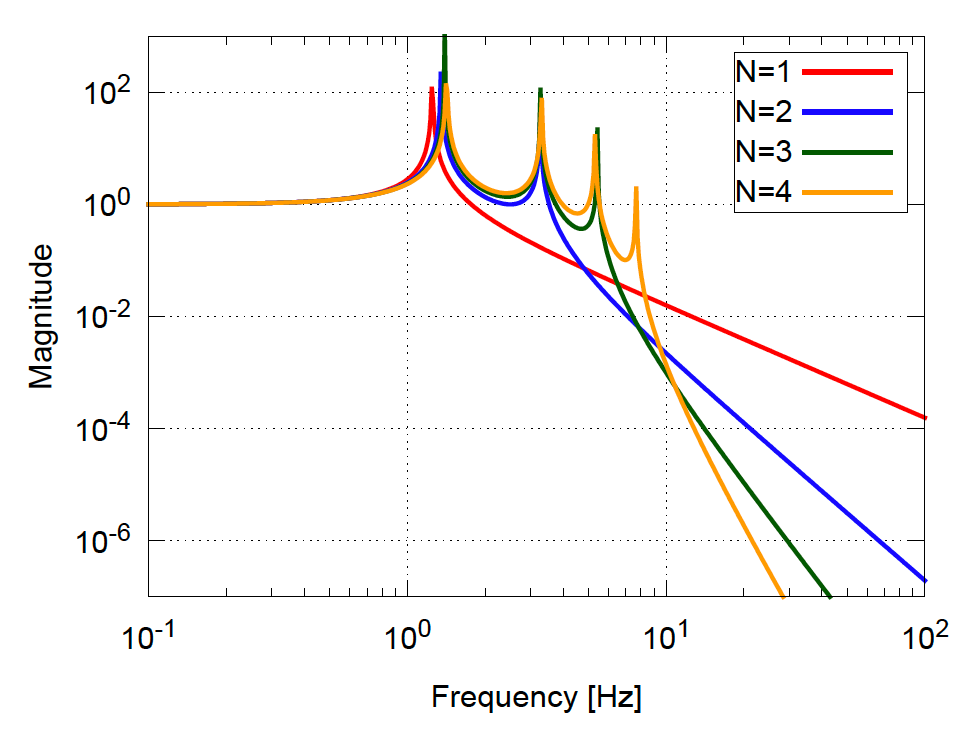
\includegraphics[width=10cm,height=7cm]{./img_chap5/img502.png}
    \caption{The amplitude of the transfer function of the N-stage pendulum. This figure is cited from Fig. 2.4 in \cite{sekiguchi2016astudy}.} \label{img:img502}
  \end{center}
\end{figure}


\section{Active Inertial Seismic Isolation}\label{sec:512}
\begin{figure}[h]
  \begin{center}
    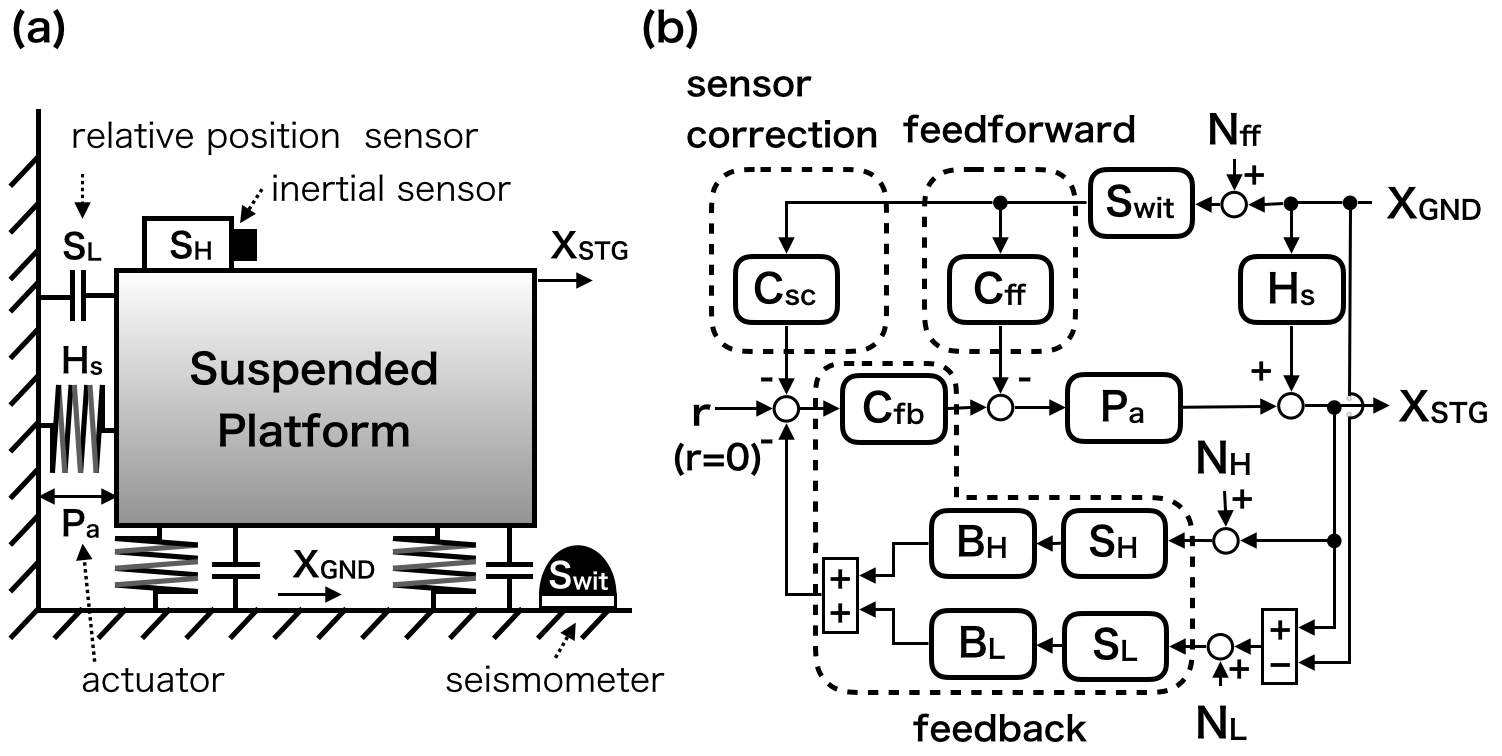
\includegraphics[width=13.5cm]{./img_chap5/img503.png}
    \caption{{\bf(a)} Schematic drawing of an active seismic isolation system for platform. {\bf(b)} Block diagram of the active control scheme.} \label{img:img503}
  \end{center}
\end{figure}
振り子をもちいた受動防振ではその共振周波数以下の地面振動は防振できない。さらに低周波で防振するために、広帯域地震計をもちいた能動防振が開発されてきた\cite{matichard2015seismic}。

The active isolation system is shown in Fig. \ref{img:img503}(a). A platform is suspended from the ground with transmisivity $H_{\mathrm{s}}$. This platfrom is fed back both signal of a inertial sensor with calibration factor $S_{\mathrm{H}}$ and signal of a relative position sensor with calibration factor $S_{\mathrm{L}}$, to the platform using actuator with actuator efficiency $P_{\mathrm{a}}$. This feedback control actively decouple the platform from the seismic disturbance from $0.1\,\mathrm{Hz}$ to a few Hz. Moreover, the platform is controled with feedforward using a seismometer with calibration factor $S_{\mathrm{wit}}$ installed on the local ground. 

能動防振の制御方法はFig.\ref{img:img503}(b)に示しているとおり、フィードバック制御、センサーコレクション制御、フィードフォワード制御、が組み合わされている。順番にそれらを説明する。

\subsection{Sensor Blending Technique}
\begin{figure}[h]
  \begin{center}   
    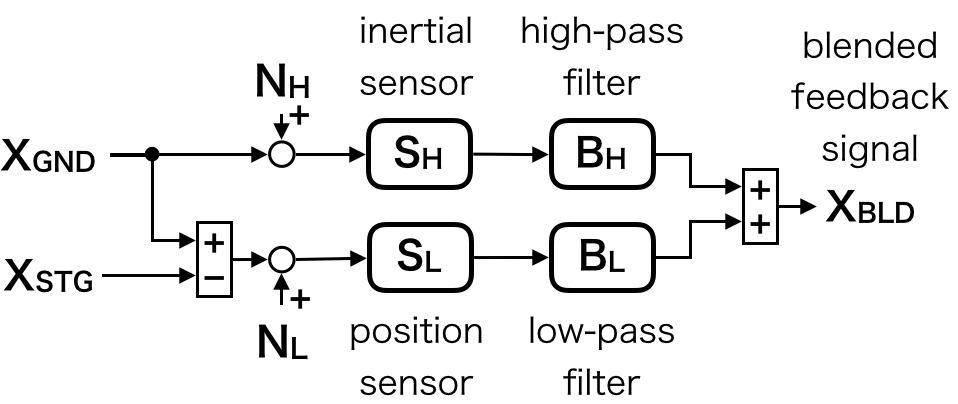
\includegraphics[width=10cm]{./img_chap5/img507.png}
    \caption{Sensor Blending.} \label{img:img507}
  \end{center}
\end{figure}

Fig.\ref{img:img507}に示すように、制御信号には慣性センサーと相対位置センサーをブレンドした信号を使う。慣性センサーは低周波で感度が悪くなるので慣性センサーにはハイパスフィルター$B_{\mathrm{H}}$をかけ、これに対して相対位置センサーには、
\begin{eqnarray}
  B_{\mathrm{H}}S_{\mathrm{H}} + B_{\mathrm{L}}S_{\mathrm{L}} = 1   \label{eq:eq506}
\end{eqnarray}
となるような相補的なローパスフィルター$B_{\mathrm{L}}$をかける。

このようにブレンドされた制御信号をつかってフィードバック制御した場合での、プラットフォームのステージの変位を考える。まず、platform のステージの変位 $X_{\mathrm{STG}}$は地面振動$X_{\mathrm{GND}}$、慣性センサーノイズ$N_{\mathrm{H}}$、相対位置センサーのノイズ$N_{\mathrm{H}}$で表すと
\begin{eqnarray}
  X_{\mathrm{STG}} = \frac{G}{1+G}LX_{\mathrm{GND}} + \frac{1}{1+G}H_{\mathrm{s}}X_{\mathrm{GND}} + \frac{G}{1+G}\left(HN_{H}+LN_{L}\right)   \label{eq:eq510}
\end{eqnarray}
のようになる。ここで、ループゲインを$G=C_{\mathrm{fb}}P_{\mathrm{a}}$、相補フィルターとそれぞれのセンサー効率の積を$L=B_{\mathrm{H}}S_{\mathrm{H}}$、$H=B_{\mathrm{L}}S_{\mathrm{L}}$として、さらに計算の途中でEq.(\ref{eq:eq506})をつかった。すなわち、フィードバック制御が十分に働いている場合、つまりループゲインの値が十分に大きいときのステージの変位は
\begin{eqnarray}
  \lim_{G\to\infty} X_{\mathrm{STG}} = LX_{\mathrm{GND}} + \left(HN_{H}+LN_{L}\right) \label{eq:eq510_a}
\end{eqnarray}
である。

Eq.(\ref{eq:eq510_a})によれば、ステージの変位を慣性系に対して防振させるためには伝達関数$L$を小さくすればよいが、これは同時に相補フィルターである$H$を大きくすることを意味し、かえって慣性センサーのノイズをステージに流入させてしまう。現実的には、ローパスフィルター$B_{\mathrm{L}}$のカットオフ周波数は$100\,\mathrm{mHz}$が限界であり、それ以下の周波数では地面振動は防振されない。別の言い方をすれば、慣性センサーをつかったフィードバック制御は、ブレンディングフィルター$L$で地面振動からステージへの応答を整えることができる一方で、低周波の感度不足によって防振できる帯域が制限される。



\subsection{Sensor Correction Technique}
\begin{figure}[h]
  \begin{center}   
    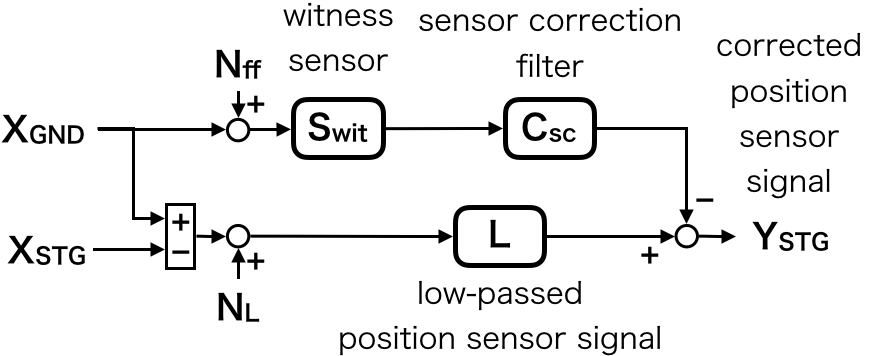
\includegraphics[width=10cm]{./img_chap5/img505.png}
    \caption{Sensor correction scheme.} \label{img:img505}
  \end{center}
\end{figure}
センサーコレクション制御は相対位置センサーを慣性センサーに修正するための方法である。\cite{hua2005low}。上述したとおり、Eq.(\ref{eq:eq506})の関係をもつ相補フィルターでブレンドされた制御信号をつかうと、慣性センサーの感度が足りない低周波帯域では、相対位置センサーの信号をつかってフィードバック制御をしなければならない。この相対位置センサーは地面からのステージの変位を測るので、低周波帯域では、ステージは地面に対して同じに動くことを意味する。そこでFig.\ref{img:img505}に示すように、もう一つ別の地面においた感度の良い地震計で測定した地面振動をつかって、変位センサーの信号から地面振動成分を取り除く。この修正された相対位置センサーの信号を制御信号につかえば、ステージに置いた慣性センサーの感度不足を補うことができる。

センサーコレクションをつかった場合のステージの変位を考える。Fig.\ref{img:img503}に示すように、センサーコレクションの信号は制御フィルター$C_{\mathrm{sc}}$を経てセットポイントで制御信号から地面振動成分を取り除く。この修正によって、ステージの変位は
\begin{eqnarray}\nonumber
  X_{\mathrm{STG}} &=&\frac{G}{1+G}L\left(1-C_{\mathrm{sc}}\frac{S_{\mathrm{wit}}}{L}\right) X_{\mathrm{GND}} + \frac{1}{1+G}H_{\mathrm{s}}X_{\mathrm{GND}}\\ 
  &+& \frac{G}{1+G}\left(HN_{H}+LN_{L}\right) + \frac{G}{1+G}C_{\mathrm{sc}}S_{\mathrm{wit}}N_{\mathrm{ff}} \label{eq:eq511}
\end{eqnarray}
のように与えられる。フィードバックが働くようにループゲインを十分大きくすると、
\begin{eqnarray}
  \lim_{G\to\infty} X_{\mathrm{STG}} = L\Delta_{\mathrm{sc}} X_{\mathrm{GND}} + \left(HN_{H}+LN_{L}\right) + {L}N_{\mathrm{ff}} \label{eq:eq513}
\end{eqnarray}
になる。ここでゲインマッチ誤差を
\begin{eqnarray}
  \Delta_{\mathrm{sc}} \equiv \left(1-C_{\mathrm{sc}}\frac{S_{\mathrm{wit}}}{L}\right) \label{eq:eq512}
\end{eqnarray}
とした。したがってEq.(\ref{eq:eq513})はEq.(\ref{eq:eq510_a}) と比較すると、ステージの変位はゲインマッチ$\Delta_{\mathrm{sc}}$によって地面振動の寄与を低減できることがわかる。

このゲインマッチは、Eq.(\ref{eq:eq512})によれば$C_{\mathrm{sc}}=B_{\mathrm{L}}(S_{\mathrm{wit}}/S_{\mathrm{L}})$のときゼロになるが、実際はWitnessセンサーとステージに置いた慣性センサーのキャリブレーションエラーで制限される。現実的にはキャリブレーションエラーはすくなくとも5\%程度になるので、センサーコレクションのみで防振比を20以上にするのは難しい\cite{hua2005low}。


\subsection{Feedforward Technique}
\begin{figure}[h]
  \begin{center}   
    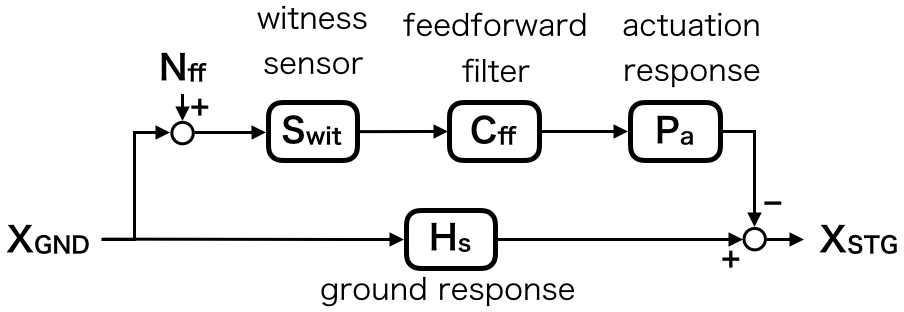
\includegraphics[width=10cm]{./img_chap5/img506.png}
    \caption{Sensor correction scheme.} \label{img:img506}
  \end{center}
\end{figure}
センサーコレクションに似た方法としてfeedforward制御がある。これはステージの地面振動揺れを直接取り除く方法である。Fig.\ref{img:img506}に示すように、地面からのステージへの伝達関数$H_{\mathrm{s}}$で伝わるステージの揺れを、地面においたWitnessセンサーで測った地面振動の信号をつかってステージを$P_{\mathrm{s}}$で動かす。このフィードフォワード制御はフィードバック制御に依らない。つまり、フィードフォワード制御はフィードバックループが小さい帯域で働き、一方でセンサーコレクション制御はフィードバックループが大きい帯域ではたらく。このような2つの制御をフィードバック制御に組み合わせることで、地面振動ノイズを低減する。

フィードフォワード制御、センサーコレクション制御、フィードフォワード制御で制御されている状態での、ステージの変位を考える。
Fig.\ref{img:img503}にしめすとおり、エラーポイントにフィードフォワード信号を、セットポイントにセンサーコレクション信号を入れる。このときのステージの変位は、
\begin{eqnarray}\nonumber
  X_{\mathrm{STG}} &=&\frac{G}{1+G}L\Delta_{\mathrm{sc}} X_{\mathrm{GND}} + \frac{1}{1+G} \Delta_{\mathrm{ff}} X_{\mathrm{GND}}\\ \nonumber
  &+& \frac{G}{1+G}\left(HN_{H}+LN_{L}\right) + \frac{G}{1+G}C_{\mathrm{sc}}S_{\mathrm{wit}}N_{\mathrm{ff}} \\ 
  &+& \frac{1}{1+G}P_{\mathrm{a}} C_{\mathrm{ff}}S_{\mathrm{wit}}N_{\mathrm{ff}} \label{eq:eq514}
\end{eqnarray}
となる。ここで新たにフィードフォワード制御でのゲインマッチ誤差
\begin{eqnarray}
  \Delta_{\mathrm{ff}} \equiv \left(H_{\mathrm{s}}-P_{\mathrm{a}}C_{\mathrm{ff}}S_{\mathrm{wit}}\right) \label{eq:eq515}
\end{eqnarray}
を導入した。Eq.(\ref{eq:eq514})において、地面振動からの寄与を表す第一項と第二項はそれぞれ、ループゲイン$G$とは独立して、$\Delta_{\mathrm{sc}}$と$\Delta_{\mathrm{ff}}$をつかって低減できることがわかる。


\subsection{Problem in Tilt-Horizontal Coupling}
\begin{figure}[h]
  \begin{center}   
    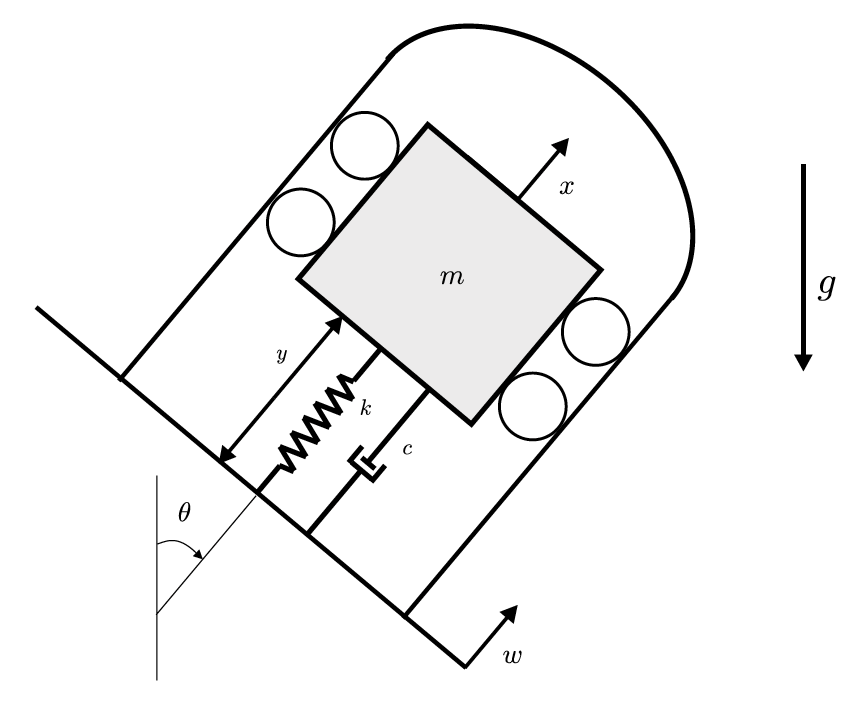
\includegraphics[width=8cm]{./img_chap5/img509.png}
    \caption{Tilted inertial sensor. Cited from Fig.12 in \cite{collette2012inertial}} \label{img:img509}
  \end{center}
\end{figure}

慣性センサーは慣性系からみた見かけの力を測るので、地面の加速度運動と傾斜による重力加速度の変化を区別することはできない。これはTilt-Horizontalカップリングとして知られ、次式のように、センサー信号は地面振動と傾斜の両方に応答してしまう\cite{collette2012inertial}。
\begin{eqnarray}
  Y(s)=\frac{-m s^{2}}{m s^{2}+c s+k} \left[ W(s) + \frac{g \sin \left(\theta_{0}\right)}{s^2} \Theta(s) \right] \label{eq:eq515}
\end{eqnarray}
ここで、$W(s),\,Y(s),\,\Theta(s)$はそれぞれラプラス空間での、振動子の変位、センサーが測る筐体と振動子との相対変位、筐体の傾斜角である。また$m,\,c,\,k,\,g,\,\theta_0$はそれぞれ、振動子の質量、粘性減衰係数、ばね定数、重力加速度、つりあいの状態での角度である。Eq.(\ref{eq:eq515})によれば、
\begin{eqnarray}
  f < \sqrt{\frac{g\sin(\theta_0)}{(2\pi)^2}}\ [\mathrm{Hz}]
  \label{eq:eq515}
\end{eqnarray}
のとき傾斜成分が卓越してくる。たとえば最も傾斜からのカップリングが大きい$\theta_0=\pi/2$のとき、つまり地面振動の並進成分は$f<0.5\ [\mathrm{Hz}]$のとき傾斜成分に埋もれてしまう。

このように低周波では傾斜計として振る舞う慣性センサーを能動防振につかうことはできない。したがって傾斜成分を別の慣性センサーで測定して、制御信号から傾斜成分を取り除くことが必要となり制御が複雑になってしまう\cite{biscans2018optimization}。





\section{Active Baseline Seismic Isolation}
レーザー干渉計型重力波望遠鏡にとって防振すべきは基線長であり、必ずしも個々のステージを慣性系に防振する必要はない。このことに着目して、Suspension Point Interferometer (SPI) と呼ばれる干渉計をつかう基線長能動防振が開発されてきた。

\begin{figure}[H]
  \begin{center}   
    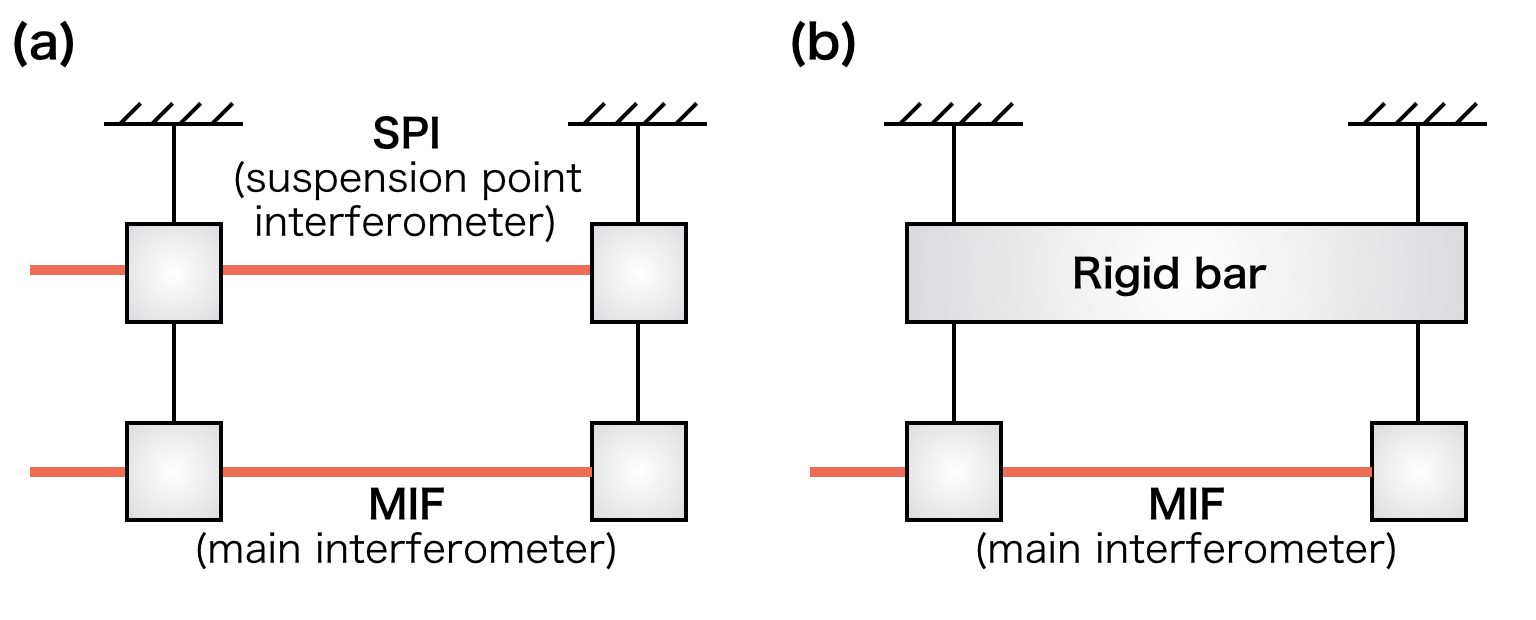
\includegraphics[width=13cm]{./img_chap5/img508.png}
    \caption{Schematic arrangement for one arm of SPI.} \label{img:img508}
  \end{center}
\end{figure}
\subsection{Suspension Point Interferometer (SPI)}
基線長能動防振のアイデアはDreverによっておよそ30年前に考案された。このアイデアは、腕共振器の懸架点間の長さを Suspension point interferometer (SPI) と呼ばれる補助光学系をつかって測り、その信号で懸架点間の距離を一定に保つように制御するというものであった\cite{drever1987outline}。慣性センサーをもちいた能動防振とは異なり、低周波で感度が良いので、SPIをもちいた能動防振はDCまで防振することができ、最大の利点である。そしてこれまでに次に述べるようなさまざまなSPIが開発されてきた。

\subsubsection{Fabry-Perot Optical Cavity Type }
まずはじめに考案されたのが、Fig.\ref{img:img508}(a) のように主干渉計の腕共振器のすぐ上の段をつかってFabry-Perot共振器をつくるアイデアである\cite{drever2002extension}。このアイデアの優れた点は、テストマスのすぐ近くで腕共振器長を測りフィードバック制御できるので、ゲインを十分に大きくすれば Fig.\ref{img:img508}(b) のように剛体棒として上段は振る舞う。これはつまり、一切基線長変動しない地面振動から単振り子で腕共振器が懸架されていることを意味し、究極的な防振である。そして程なくして、2mの大きさのプロトタイプが開発され、主干渉計の腕共振器長変動を$1\,\mathrm{Hz}$以下で$40\,\mathrm{dB}$低減することが実証された\cite{aso2004stabilization}。

しかしながら、section \cref{sec532} で後述する通り、SPIは共振器長変動のみをモニターしてフィードバック制御するので、腕共振器全体が動くような地面振動の同相成分を低減することができない。言い換えると、SPI以下の振り子の対称性が悪くCMRRが悪いと地面振動の同相成分は共振器長変動にカップリングしてしまう。このことから振り子の共振周波数以上ではCMRRによって能動防振の性能は制限される。

さらにFabry-Perot光共振器型のSPIだと線形レンジが小さいため、SPI自身が共振するためにRMSをおさえるための防振が必要であり、SPI自身の動作が不安定である。2mのプロトタイプでは基線長が短いため、section \cref{sec:sec313} で述べたように、地面振動の逆相成分は十分小さく低減されているが、kmスケールのFabbry-Perot光共振器型のSPIを安定して動作させるには、1000倍条件が厳しくなる。また長期線になれば角度制御に対する要求値も厳しくなるため、Fabry-Perot光共振器型のSPIは問題をかかえてしまう。

\subsubsection{Homodyne Michelson Interferometer Type}
\begin{figure}[h]
  \begin{center}   
    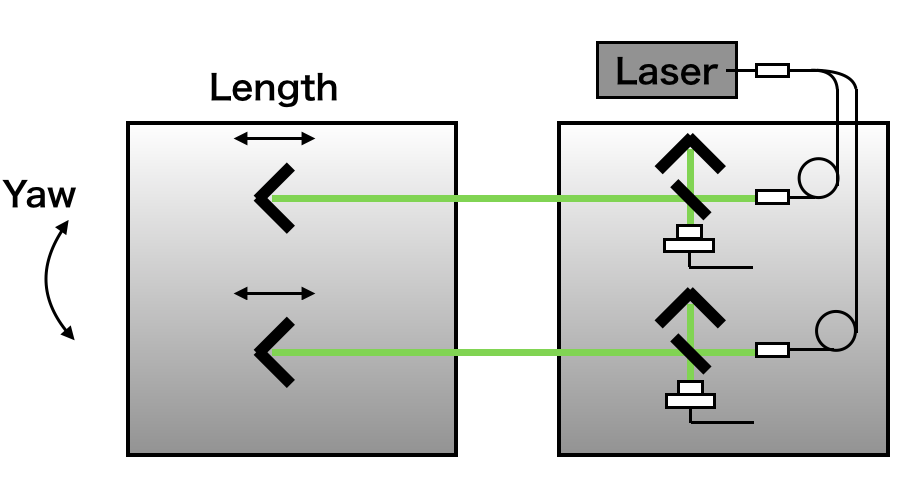
\includegraphics[width=9cm]{./img_chap5/img508a.png}
    \caption{Active baseline seismic isolation system using Michelson Type SPI \cite{Numata2008interferometric}. 2つのSPIで基線方向とYaw方向の制御をしている。それぞれのSPIはエンド鏡にコーナーキューブを使用している非対称マイケルソン干渉計であり、干渉信号はホモダイン検波で取得している\cite{araya2002iodine}。コーナーキューブは干渉させるためのアラインメント調整を必要としないが、その反面、角度変化と基線変化を区別できないので、SPIが2台必要になる。} \label{img:img508a}
  \end{center}
\end{figure}
測定のレンジが非常に狭いFabry-Perot光共振器の問題を解決するために、Michelson干渉計をSPIに使った能動防振が開発された\cite{Numata2008interferometric}。このMichelson干渉計はGIFと同じ構成となっており、1m離れたステージ間の距離を一定にたもつようフィードバック制御した。その結果、数時間以上にわたって数nmスケールで基線長を防振することを実証した。

しかしながら、エンドミラーにコーナーキューブを使用しており、角度変化と基線長変化を区別できないため、それらを分離するためにさらに余分にSPIを必要とする。この研究では、YAW方向のみ制御するために合計で2台のSPIをつかっていたが、PIT成分も分離するためには合計で3台のSPIが必要である。実際、彼らの能動防振ではPITの角度揺れからのカップリングが低周波の防振を制限していたため、3台目のSPIが必要である。

\subsubsection{Heterodyne Mach-Zehnder Interferometer Type}
SPIで角度制御するために


\cite{dahl2012suspension,sina2018towards}

\subsection{Limitation due to CMRR}\label{sec532}
\begin{figure}[h]
  \begin{center}   
    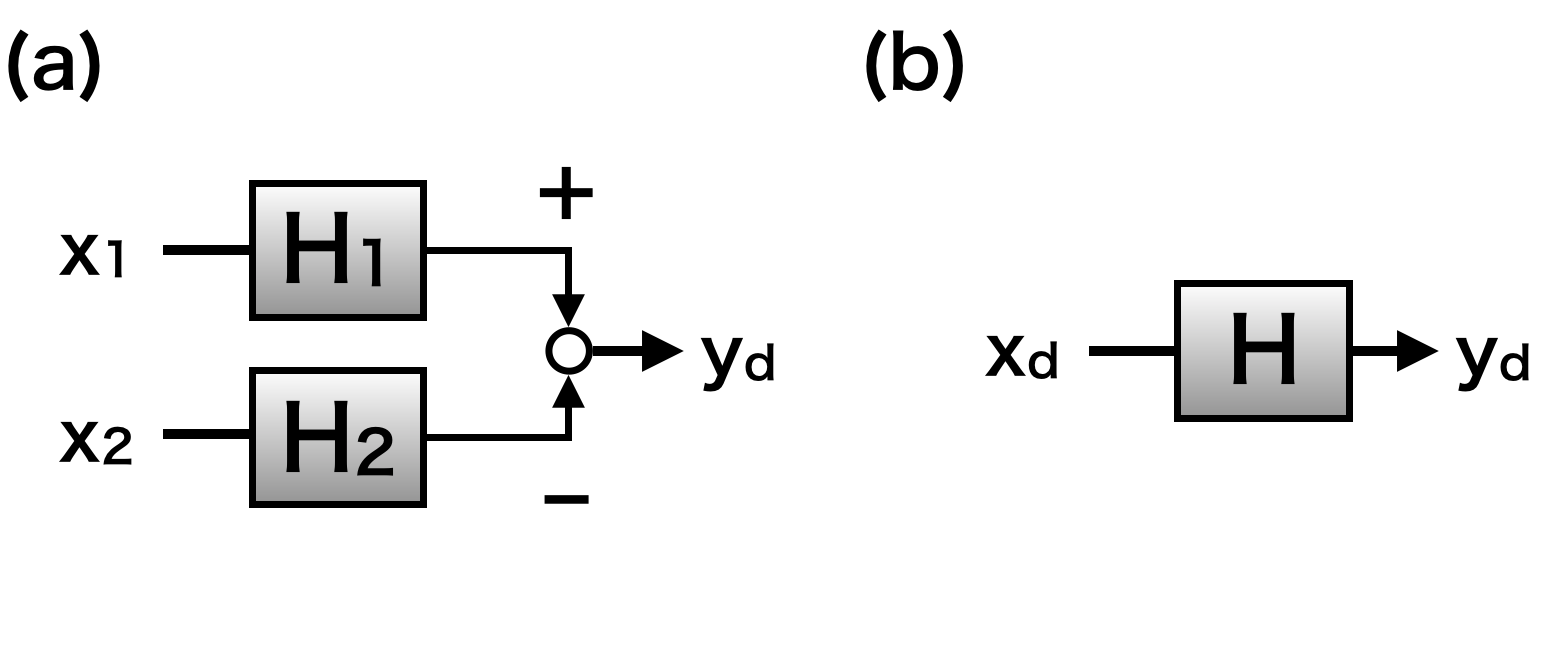
\includegraphics[width=10cm]{./img_chap5/img510.png}
    \caption{...} \label{img:img510}
  \end{center}
\end{figure}
Section \cref{sec:512} で述べた能動防振は同相成分と逆相成分の両方を防振していたのに対して、SPIを使う能動防振では同相成分は防振しない。つまり同相雑音除去比が悪いと同相成分の地面振動がステージ間の相対変位にカップルしてしまう。

同相成分から差動成分への寄与を考える。Fig.\ref{img:img510}(a)のように、2つの場所での地面振動$x_1,\,x_2$がそれぞれの防振ステージの伝達関数$H_1,\,H_2$を経て、ステージの相対変位$y_d$として出力される、2入力1出力のシステムを考える。それぞれのステージと地面振動の変位を$X_{i},\,x_{i}$とし、地面からステージへの伝達関数を$H_{i}$とする。ここで添字は$i=1,2$であり、それぞれITMXとETMXを表す。つまりステージの相対変位$X_{\mathrm{d}}$は
\begin{eqnarray}
  y_{\mathrm{d}} = H_1x_1-H_2x_2 \label{eq:eq517}
\end{eqnarray}
である。ここでこれら伝達関数と地面振動について差動成分と同相成分を
\begin{eqnarray}
  x_{\mathrm{d}} = {x_1-x_2},\ x_{\mathrm{c}} = {x_1+x_2}  \\
  H_{\mathrm{d}} = \frac{H_1-H_2}{2},\ H_{\mathrm{c}} = \frac{H_1+H_2}{2} \label{eq:eq517_a}
\end{eqnarray}
のように定義し、Eq.(\ref{eq:eq517})を新しく書き下せば、
\begin{eqnarray}
  y_{\mathrm{d}} &=& H_1x_1-H_2x_2 \\
  &=& H_{\mathrm{c}}x_{\mathrm{d}} + H_{\mathrm{d}}x_{\mathrm{c}}\label{eq:eq516}
\end{eqnarray}
のようにステージの差動信号は地面振動の差動信号と同相信号で表すことができるが、ここでこの差動システムのCMRRを
\begin{eqnarray}
  H_{\mathrm{CMRR}} \equiv \frac{H_1+H_2}{H_1-H_2}=\frac{H_{\mathrm{c}}}{H_{\mathrm{d}}} \label{eq:eq519}
\end{eqnarray}
と定義すれば、差動システムは
\begin{eqnarray}
  y_{\mathrm{d}} = H_{\mathrm{c}}\left( x_{\mathrm{d}} + \frac{1}{H_{\mathrm{CMRR}}}x_{\mathrm{c}}\right) \label{eq:eq518}
\end{eqnarray}
となる。つまりEq.(\ref{eq:eq518})は、CMRRを十分おおきくすれば地面振動の同相成分からの寄与を小さくできることを意味している。言い換えるとCMRRの逆比は地面の同相成分から差動成分へのカップリングをあらわしている。

このCMRRは2つの防振装置の差に敏感であるため、共振周波数がわずかにずれると共振周波数以上ではCMRRは悪化する。たとえばEq.(\ref{eq:eq502})のように単振り子だとした場合、高周波では$H\sim{({f_0}/{f})^2}$の伝達関数をもつ。このとき共振周波数が$\Delta{f_0}$ずれると、高周波では$2f_0\Delta{f_0}$ほどゲインに違いが生じる。これはそのままCMRRを悪化させ、高周波での防振比を制限する。


\subsection{差動能動防振システム}
\begin{figure}[h]
  \begin{center}   
    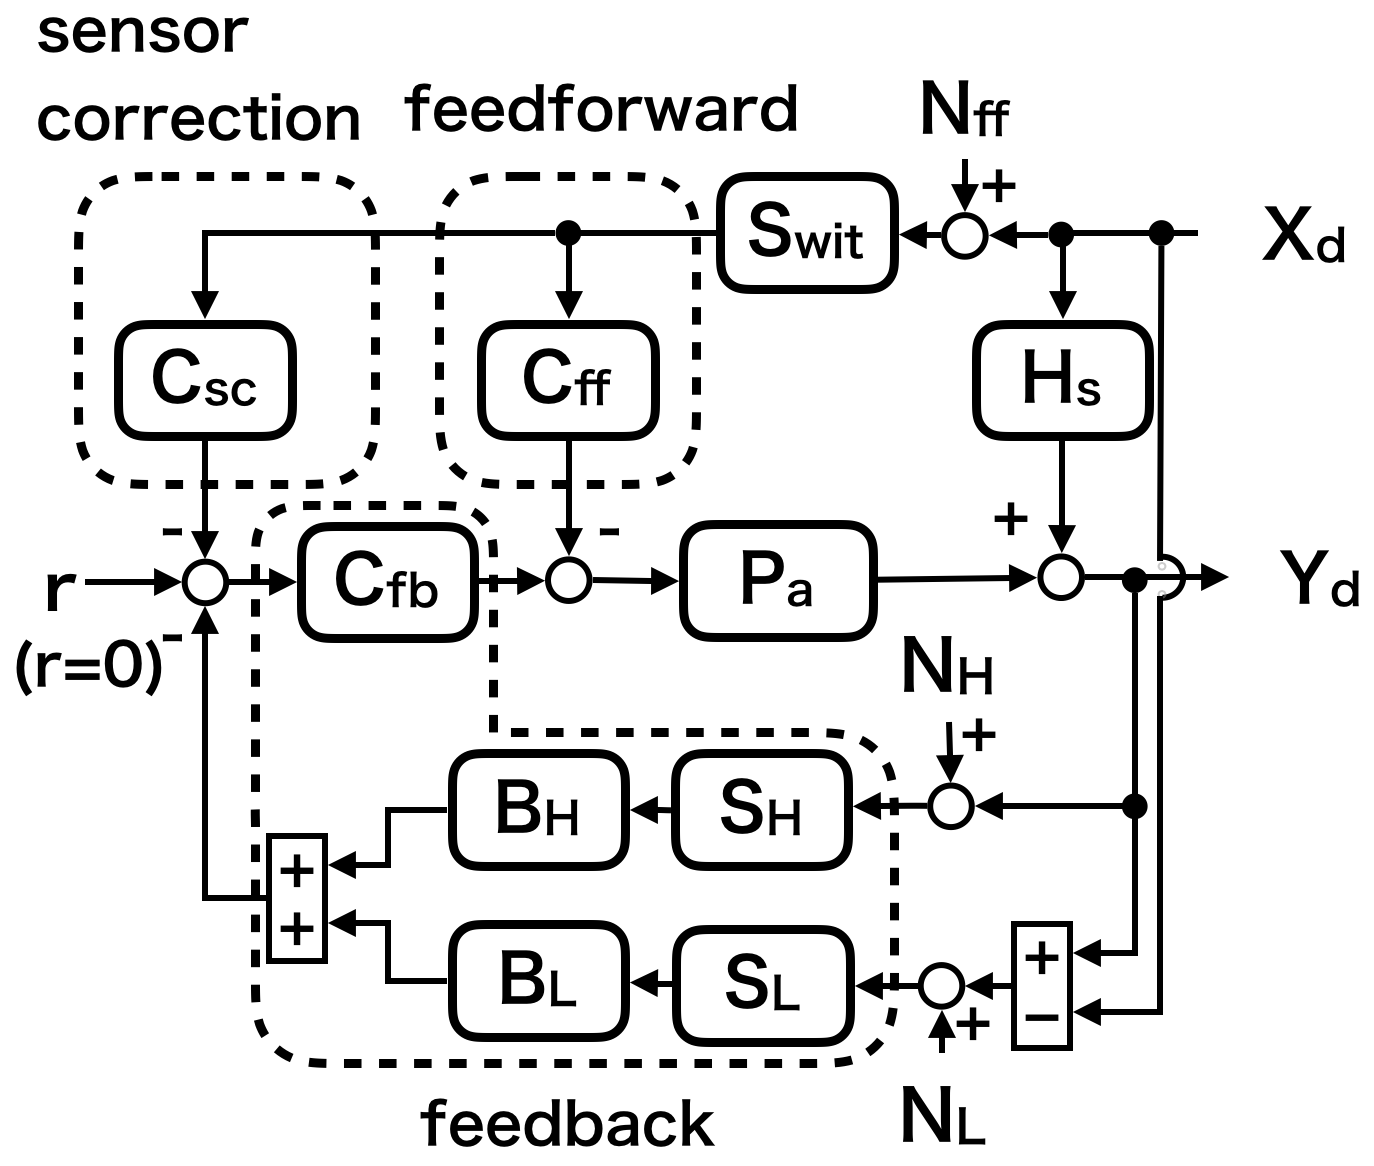
\includegraphics[width=10cm]{./img_chap5/img511.png}
    \caption{SPIをつかったステージの相対変位の能動防振。$X_{\mathrm{d}},\,X_{\mathrm{c}}\,[\mathrm{m}]$はそれぞれ地面振動の差動成分と同相成分である。$H_{\mathrm{d}},\,H_{\mathrm{c}}\,[\mathrm{m/m}]$はEq.(\ref{eq:eq517_a})で定義される伝達関数である。$S_{\mathrm{SPI}}\,[\mathrm{V/m}],\,C_{\mathrm{f}}\,[\mathrm{V/V}],\,P\,[\mathrm{m/V}]\,\,N_{\mathrm{SPI}}\,[\mathrm{m}]$はそれぞれ、SPIのセンサー効率、フィードバックフィルター、アクチュエータからステージの差動揺れへの伝達関数、SPIのセンサーノイズである。} \label{img:img511}
  \end{center}
\end{figure}
Fig.\ref{img:img511}に示すような制御でSPIをつかってステージの差動成分$Y_{\mathrm{d}}$を防振する。このときの差動成分は、
\begin{eqnarray}
  Y_{\mathrm{d}}=\frac{1}{1+G} \left( H_{\mathrm{c}} X_{\mathrm{d}} + H_{\mathrm{d}}X_{\mathrm{c}} \right) + \frac{G}{1+G} N_{SPI}
\end{eqnarray}
となる。ここでループゲインを$G=S_{\mathrm{SPI}}C_{\mathrm{fb}}P$とした。

\subsection{RMS Reduction}
SPIをつかえば腕共振器長のRMSを低減することができる。

腕共振器のRMSが小さくなれば後述するとおり、重力波望遠鏡にとってさまざまな利点を与える。

\subsubsection{Improvement of Actuator Noise}
腕共振器のRMSが小さくなることで、テストマスのアクチュエータ効率を小さくでき、アクチュエータ雑音を小さくすることができる。

\subsubsection{Improvement of Glitch Noise}
腕共振器のRMSが小さくなることで、アクチュエータにかかる電圧値を小さくでき、バルクハウゼンノイズを低減することが期待できる。

\cite{manson1972frequency}
\cite{aasi2015characterization}
\cite{cote1991self}

\subsubsection{Facilitation of Lock Acquision}
腕共振器のRMSが小さくなることで、ロックアクイジションが容易になる。

\subsection{Some Difficulties}
\subsubsection{Difficulty due to Asymmetry of the Suspensions}
SPIをつかった能動防振は共振器長さを一定にたもつように制御するので、腕共振の同相の動きは防振できない。このとき、サスペンションの非対称性から同相雑音除去比が悪いと、この同相成分が腕共振器長にカップルしてしまう。

\subsubsection{Difficulty in Large Scale GW detectors}
SPIの欠点は、建設のコストとアラインメントの難しさにある。





%
\section{Baseline Compensation System}\label{sec:52}
\subsection{Concept}
SPIをつかった能動防振の防振性能はCMRRで決まるため、CMRRが悪くなる共振周波数以上の帯域では能動防振をしない。


\subsection{Advanatge of GIF}
\subsection{GIF as SPI}
\subsection{Control Scheme}



\section{Summary of the Chapter}
